% Conference paper -- Where the Map Disagrees:
% Disagreement-Guided Discovery of New Periodic Orbits in the Three-Body Problem.
%
% Target venues: NeurIPS workshop on ML for the Physical Sciences,
% AIP Chaos, or Phys. Rev. Research.
%
% Alternative title (if a venue prefers a more conservative phrasing):
% Alternative: Label-Disagreement Active Learning Discovers New Periodic Orbits in the Three-Body Problem

\documentclass[10pt]{article}
\usepackage[a4paper,margin=1in]{geometry}
\usepackage[utf8]{inputenc}
\usepackage[T1]{fontenc}
\usepackage{lmodern}
\usepackage{microtype}
\usepackage{amsmath,amssymb}
\usepackage{mathtools}
\usepackage{booktabs}
\usepackage{graphicx}
\graphicspath{{figures/}}
\usepackage{caption}
\captionsetup{font=small,labelfont=bf,labelsep=period,skip=4pt}
\usepackage[numbers,sort&compress]{natbib}
\usepackage{hyperref}
\hypersetup{
  colorlinks=true,
  linkcolor=blue!55!black,
  citecolor=teal!60!black,
  urlcolor=blue!55!black,
  pdftitle={Disagreement-Guided Discovery of Periodic Orbits in the Three-Body Problem}
}
\usepackage{xcolor}
\usepackage{titlesec}
\titleformat{\section}{\large\bfseries}{\thesection}{0.7em}{}
\titleformat{\subsection}{\normalsize\bfseries}{\thesubsection}{0.7em}{}
\titlespacing{\section}{0pt}{0.9\baselineskip}{0.3\baselineskip}
\titlespacing{\subsection}{0pt}{0.55\baselineskip}{0.2\baselineskip}

% Tighten float behaviour so figures land near their references.
\renewcommand{\topfraction}{0.92}
\renewcommand{\bottomfraction}{0.85}
\renewcommand{\textfraction}{0.05}
\renewcommand{\floatpagefraction}{0.85}
\setcounter{topnumber}{3}
\setcounter{bottomnumber}{2}
\setcounter{totalnumber}{5}
\setlength{\textfloatsep}{8pt plus 2pt minus 2pt}
\setlength{\floatsep}{8pt plus 2pt minus 2pt}
\setlength{\intextsep}{8pt plus 2pt minus 2pt}
\setlength{\abovecaptionskip}{4pt}
\setlength{\belowcaptionskip}{2pt}

\setlength{\parskip}{0.3em}
\setlength{\parindent}{1.2em}

% Compact macros
\newcommand{\vvec}{\mathbf{v}}
\newcommand{\xvec}{\mathbf{x}}
\newcommand{\qvec}{\mathbf{q}}
\newcommand{\pvec}{\mathbf{p}}
\newcommand{\Norm}[1]{\left\lVert#1\right\rVert}
\newcommand{\RR}{\mathbb{R}}
\newcommand{\Tstar}{T^{\star}}

\title{\bfseries Where the Map Disagrees:\\
  Disagreement-Guided Discovery of New Periodic Orbits\\
  in the Three-Body Problem}
\author{Anonymous\\\small (author and affiliation omitted for blind review)}
\date{}

\begin{document}
\maketitle

\begin{abstract}
\noindent A neighbourhood-disagreement prior discovers $2.4\times$ more
periodic orbits per unit compute than classifier-entropy baselines
(paired $t = 38$, $p = 1.5\!\times\!10^{-11}$, ten seeds) in the equal-mass
planar three-body problem. Guided search identifies four orbits in the
Euler velocity section: two match Hristov \& Dmitra\v{s}inovi\'c (2025)
stable-orbit catalog entries at $50$-digit precision --- an independent
rediscovery validating the pipeline from a different starting point ---
and two are not in any published catalog of $24{,}582$ free-fall or
$971$ stable orbits. One of the unmatched orbits has a syzygy
free-group word $(132)^{8}$ absent from the $971$-label
stability-filtered topology catalog, suggesting a new family. All
orbits close to residual $<10^{-47}$ under two independent
high-precision integrators (heyoka $200$-bit MPFR Taylor and
\texttt{mpmath} pure-Python Taylor at $30$ dps), ruling out
integrator-specific spurious closure. The catalog cross-check also
exposes a previously undocumented convention discrepancy in the
Hristov (2025) catalog --- columns are Euler $(v_1, v_2, T, \Tstar)$ and
not the free-fall $(x_3, y_3, T, \Tstar)$ that the README states ---
which is invisible at $4$-digit comparison but collapses at
$50$-digit identity.
\end{abstract}

% =================================================================
\section{Introduction}

The three-body problem --- three point masses moving under mutual
Newtonian gravity --- is the historical archetype of deterministic
chaos. Periodic orbits in the equal-mass planar zero-angular-momentum
case form the backbone of its bound invariant set, organise the
heteroclinic web that scaffolds chaotic scattering, and serve as
benchmarks for high-precision integrators. Catalogs of such orbits have
grown by enumeration: \citet{Suvakov2013} produced thirteen families by
hand-tuned grid search in $(v_1, v_2)$; the Li--Liao group at Shanghai
Jiao Tong combined symplectic shooting with grid search to extend this
to $695$~families \citep{LiLiao2017}; and \citet{Hristov2024Catalog}
pushed the catalog to $12{,}409$ distinct free-fall orbits ($24{,}582$
initial conditions including duals) at scale-invariant period
$\Tstar < 80$. \citet{Hristov2025Stable} filtered that catalog for
linear stability, yielding $971$ stable orbits.

Two trends in this literature motivate the present work. First, the
classical hand-search strategy --- pick a family-specific symmetry,
grid the invariant parameters --- relies on structural ansatzes and
will miss orbits whose symmetries are not anticipated. Second, recent
work on escape-basin structure \citep{Trani2024, Manwadkar2021} shows
that ``isles of regularity'' --- bounded phase-space regions punctuated
by periodic orbits --- concentrate on multi-class Wada boundaries
\citep{GOY1983, MGOY1985, Aguirre2001, Poon1996, NusseYorke1992}.
A learned surrogate of basin structure should therefore be a stronger
prior for periodic-orbit search than uniform sampling, provided one can
extract a signal that \emph{localises the boundary skeleton} rather
than merely flagging classifier uncertainty.

The point of departure for this paper is a small but consequential
distinction. Where a basin classifier is \emph{uncertain} ---
high-entropy in its softmax --- the locus is noisy and includes diffuse
interior regions. Where its \emph{neighbours disagree on the hard
label} --- a $k$-NN statistic on the labelled training grid --- the
locus is specifically the basin boundary. The two families of
uncertainty are different in principle (epistemic vs.\ aleatoric, in
effect) and very different in practice. We make this distinction
explicit, derive a label-disagreement prior $D_k(\vvec)$, and run a
ten-seed paired-design ablation against the standard classifier-entropy
baseline.

\paragraph{Contributions.}
(i)~A label-disagreement prior for ML-guided periodic-orbit discovery,
grounded in basin-boundary theory.
(ii)~A ten-seed paired-design study showing $D_k$ outperforms entropy
by $2.4\times$ in verified-orbit yield ($p = 1.5\!\times\!10^{-11}$,
Cohen's $d = 12.0$, win rate $10/10$).
(iii)~Discovery and high-precision verification of four periodic
orbits, two of which are independent rediscoveries of Hristov 2025
entries (validating the pipeline) and two of which are absent from
published catalogs; all close below $10^{-47}$ under two independent
integrators.
(iv)~A topological classification by syzygy free-group words
establishing that one of the new orbits has a topology absent from the
$971$ published stability-filtered labels.
(v)~A previously unreported convention discrepancy in the Hristov (2025)
catalog: columns are $(v_1, v_2, T, \Tstar)$ in Euler convention, not
$(x_3, y_3, T, \Tstar)$ in free-fall convention as the README states.
The discrepancy is invisible at $4$-decimal precision but collapses to
exact identity at $50$ digits.

% =================================================================
\section{Related Work}

\paragraph{Numerical orbit catalogs.}
\citet{Moore1993} introduced the figure-eight braid and
\citet{ChencinerMontgomery2000} proved its existence.
\citet{Suvakov2013} produced thirteen families by hand-tuned search.
\citet{LiLiao2017} extended this to $695$ families with grid search and
symplectic shooting at the Euler velocity section. The Hristov group
\citep{Hristov2024Catalog} pushed the free-fall catalog to $12{,}409$
distinct orbits and the stable subset \citep{Hristov2025Stable} to
$971$. Both Hristov works publish initial conditions to $80$ decimal
digits.

\paragraph{Basin-boundary theory in dynamical systems.}
\citet{GOY1983, MGOY1985} introduced the fractal-basin-boundary
framework. \citet{NusseYorke1992} established the Wada-property
characterisation of multi-basin meeting curves; \citet{Poon1996}
extended it to chaotic scattering. \citet{Aguirre2001} showed that the
H{\'e}non--Heiles system has Wada boundaries with three-class meeting
points; \citet{Daza2016, Daza2018} introduced quantitative tools
(basin entropy, the merging method) for diagnosing them. The point we
build on is that the deepest such intersections in a multi-class basin
map are precisely where periodic orbits accumulate.

\paragraph{Machine learning in celestial mechanics.}
\citet{Breen2020} trained a residual MLP on chaotic three-body
trajectories. \citet{Liao2022} surveyed ML-aided periodic-orbit search
via classification of escape outcomes. \citet{Manwadkar2021} established
the L\'evy-flight statistics of bound triples and \citet{Trani2024}
mapped isles of regularity in the velocity section.
\citet{Shena2021, Valle2024} learned basin classifiers for general
dynamical systems. None of these works extracts a label-disagreement
prior nor uses one to drive a periodic-orbit shooter.

\paragraph{Active learning and uncertainty priors.}
Entropy-based active learning is a standard acquisition strategy.
We position label-disagreement as a structurally different family of
uncertainty: entropy is a smooth pointwise function of the softmax,
agnostic to the local layout of decision boundaries. Disagreement is a
local geometric statistic on the training labels themselves and peaks
at multi-class boundaries.

% =================================================================
\section{Method}
\label{sec:method}

\subsection{Problem setup}

Three point masses $m_i = 1$ ($i = 1, 2, 3$) move in the plane under
Newtonian gravity with $G = 1$. With positions $\qvec_i \in \RR^2$ and
momenta $\pvec_i \in \RR^2$, the Hamiltonian is
\begin{equation}
  H(\qvec, \pvec) = \sum_{i=1}^{3} \frac{\Norm{\pvec_i}^2}{2}
  - \sum_{i<j} \frac{1}{\Norm{\qvec_i - \qvec_j}}.
  \label{eq:ham}
\end{equation}
We enforce zero centre of mass $\sum_i \qvec_i = 0$, zero total
momentum $\sum_i \pvec_i = 0$, and zero total angular momentum
$\sum_i \qvec_i \times \pvec_i = 0$.

\paragraph{Euler velocity section.}
The pipeline searches the Euler section \citep{LiLiao2017}: bodies at
$\qvec_1(0) = (-1, 0)$, $\qvec_2(0) = (+1, 0)$, $\qvec_3(0) = (0, 0)$,
with momenta $\pvec_1(0) = \pvec_2(0) = (v_1, v_2)$ and
$\pvec_3(0) = -2(v_1, v_2)$. The two scalars $(v_1, v_2)$ parametrise
the section; a periodic orbit is the triple $(v_1, v_2, T)$ with
period $T$. The energy is $E = 3(v_1^2 + v_2^2) - 5/2$, and the
scale-invariant period is $\Tstar = T \, |E|^{3/2}$.

\subsection{Basin map and classifier}

A $500\!\times\!500$ grid in $(v_1, v_2) \in [-0.8, 0.8]^2$ is
integrated at float64 precision with a sixth-order symplectic Yoshida
integrator \citep{Yoshida1990} at step $h = 0.002$ until either (a) one
of the three pairs has positive two-body energy and is separating from
the third body --- a labelled \emph{escape} of body $i$ --- or (b) the
horizon $t_{\max} = 500$ is reached, in which case the cell is
labelled \emph{bound}. The resulting four-class label field
$y(\vvec) \in \{1, 2, 3, B\}$ is the ground truth for classifier
training; the bound region occupies $\sim\!12.6\%$ of the square and
contains all known Li--Liao $695$ families.

\begin{figure}[!htb]
\centering

\includegraphics[width=0.86\linewidth]{basin_combined_paper.pdf}
\caption{Four-way escape partition (left) and classifier softmax
entropy (right) on the velocity section
$(v_1, v_2) \in [-0.8, 0.8]^2$. Colours encode which body escapes
(or \emph{bound}, grey, $\sim\!12.6\%$ of the square). Boundaries
between escape channels are fractal (Wada). Entropy (right) saturates
on the boundary skeleton but also on locally noisy interior regions; a
label-disagreement field (not shown) concentrates instead on the
boundary curves where the ground-truth label changes class.}
\label{fig:basin}
\end{figure}

The classifier is a four-layer MLP with Fourier-features input
($K = 32$ frequencies $\omega_k \sim \mathcal{N}(0, \sigma^2 I)$,
$\sigma = 4$), three hidden layers of width $128$ with ReLU
activations, and a softmax-over-$4$ output:
\begin{equation}
  f_\theta(\vvec) = \mathrm{softmax}\!\bigl(\mathrm{MLP}_{128}^{(3)}(
  \mathrm{FF}_K(\vvec))\bigr) \in \Delta^3.
  \label{eq:mlp}
\end{equation}
Training uses categorical cross-entropy, Adam at learning rate
$10^{-3}$, $100$ epochs, and a $70/30$ stratified split. Holdout
accuracy is $91$--$94\%$. The Fourier-features layer is essential: a
raw-coordinate MLP at the same width cannot represent the
high-frequency fractal labelling. Figure~\ref{fig:basin} shows the
four-class basin map and the classifier softmax-entropy field.

\subsection{Candidate priors}

Given a candidate pool of $N = 5000$ points drawn i.i.d.\ from
$U([-0.8, 0.8]^2)$, each receives a score under one of four priors.

\paragraph{Uniform random.} Score drawn i.i.d.\ from $U(0,1)$.
\paragraph{Physics symmetry grid.} Distance to the Suvakov-type
one-parameter symmetry axes, with Gaussian reweighting of width
$\sigma = 0.03$.
\paragraph{Classifier softmax entropy (baseline ML prior).}
\begin{equation}
  H(\vvec) = -\sum_{c=1}^{4} f_\theta(\vvec)_c \,\log f_\theta(\vvec)_c.
  \label{eq:entropy}
\end{equation}
$H$ saturates near $\log 4 \approx 1.386$ wherever the softmax is
diffuse, including at boundaries but also at locally noisy interior
points.
\paragraph{$k$-NN label disagreement (ours).}
For each candidate $\vvec$, locate its $k$ nearest training-grid
neighbours $\mathcal{N}_k(\vvec)$ with hard labels $\{y_j\}$, and
define
\begin{equation}
  D_k(\vvec) \;=\; 1 \;-\; \frac{n_{\mathrm{mode}}}{k},
  \qquad
  n_{\mathrm{mode}} \;=\; \bigl| \{\, j \in \mathcal{N}_k(\vvec) :
    y_j = \mathrm{mode}(y_{\mathcal{N}_k}) \,\} \bigr|.
  \label{eq:disagreement}
\end{equation}
$D_k$ is bounded by $1 - 1/k$ (here $5/6$ for $k = 6$); it equals zero
in label-pure regions and saturates at multi-class meeting points.
Crucially, $D_k$ is not derived from the softmax: it uses the hard
ground-truth labels of the training grid directly, so it is sensitive
to the layout of the basin boundaries themselves rather than to
classifier temperature.

The top $50$ candidates under each prior, subject to a repulsion radius
$|\Delta \vvec| > 0.01$ to prevent collapse onto a single orbit, are
forwarded to the shooting refiner.

\subsection{Shooting and Levenberg--Marquardt refinement}

Each selected $\vvec_0$ is integrated under Yoshida-$6$ at $h = 0.002$
until the trajectory returns within $\Norm{\qvec(t) - \qvec(0)} < 0.1$
of its initial configuration; the candidate return time $T_0$ seeds a
Levenberg--Marquardt refiner that minimises the closure residual
\begin{equation}
  R(v_1, v_2, T) \;=\; \bigl\lVert \xvec(T; v_1, v_2) - \xvec(0; v_1, v_2) \bigr\rVert_2,
  \quad \xvec \in \RR^{12},
  \label{eq:closure-residual}
\end{equation}
over $(v_1, v_2, T)$ via finite-difference Jacobian at step
$\delta = 10^{-6}$ with $N_{\mathrm{ref}} = 10^{4}$ symplectic substeps.
A candidate is provisionally verified when $R < 10^{-10}$ within
$\le\!50$ Levenberg--Marquardt iterations; we additionally require the
residual to plateau at the double-precision floor under a resolution
stress-test
$N_{\mathrm{ref}} \in \{10^4, 3\!\times\!10^4, 10^5, 3\!\times\!10^5, 10^6\}$,
which rejects long-lived near-periodic trajectories that masquerade as
orbits at one step size.

\subsection{High-precision verification}
\label{sec:hp}

Surviving candidates are lifted from float64 to $50$ decimal digits by
Newton iteration around a heyoka \citep{heyoka} adaptive-step Taylor
integrator at $200$-bit MPFR precision in compact-mode JIT. The
period-$T$ return map and its $12 \times 3$ Jacobian
$\partial \xvec(T)/\partial(v_1, v_2, T)$ are formed by
finite-differences at step $\delta_{\mathrm{HP}} = 10^{-18}$, and the
update is the Newton--Moore--Penrose step
\begin{equation}
  (v_1, v_2, T)_{n+1} \;=\; (v_1, v_2, T)_{n}
   \;-\; J^{+} \,\bigl[\xvec(T) - \xvec(0)\bigr]_{n}.
  \label{eq:newton}
\end{equation}
Each step gains $6$--$7$ digits (quadratic convergence) and the loop
terminates when $R$ stabilises near the implementation floor
$\sim\!10^{-50}$. To rule out integrator-specific spurious closure,
every candidate is re-verified with an independent pure-Python
\texttt{mpmath} Taylor integrator at $30$ decimal digits. The two
integrators share no code: heyoka uses symbolic compilation to
MPFR-compiled assembly; the mpmath path uses recursive Python
forward-differencing. Agreement of the two implementations to better
than $5 \times 10^{-48}$ on the closure residual eliminates the
Jacobian-finite-difference and underflow loopholes.

\subsection{Catalog cross-checks and topology}
\label{sec:catalog-checks}

For each verified orbit, three external checks are performed.

\paragraph{Hristov 2024 forward-integration sweep.}
The $24{,}582$ Hristov 2024 free-fall initial conditions
\citep{Hristov2024Catalog} are not directly comparable to our
Euler-section ICs: a generic periodic orbit visits one section but not
both. We therefore forward-integrate every catalog entry under
Yoshida-$6$, scan the trajectory for collinear Euler crossings, and
apply the canonical scale transformation $\lambda = 2/d_{\mathrm{half}}$
with $T_{\mathrm{can}} = \lambda^{3/2}\, T_{\mathrm{Hristov}}$. The
closest $(v_1, v_2, T_{\mathrm{can}})$ to each of our orbits is
recorded, under the four sign symmetries
$\vvec \mapsto (\pm v_1, \pm v_2)$. A STRONG match requires
$|\Delta \vvec| < 10^{-4}$ and $|\Delta T|/T < 10^{-3}$; a WEAK match
relaxes both to $10^{-2}$.

\paragraph{Hristov 2025 direct identity check.}
The $971$ Hristov 2025 stable entries are compared at $50$-digit
precision against each of our orbits, after recognising that the
catalog columns are in Euler convention (see \S\ref{sec:hristov} for
the convention finding).

\paragraph{Topology via syzygy words.}
A \emph{syzygy} is a configuration where the three bodies are
collinear; between consecutive syzygies one of the three bodies is the
midpoint of the line. The \emph{syzygy word} of a periodic orbit is
the sequence of midpoint-body labels $\{1, 2, 3\}$ over one period.
Two orbits share a topological family iff their words are equivalent
under the free-group quotient by cyclic rotation, body permutation
$\sigma \in S_3$, and time reversal \citep{Moore1993, Montgomery2015}.
We detect syzygies by sign changes of the shape-sphere signed-area
coordinate $w = (\qvec_1 - \qvec_3) \times (\qvec_2 - \qvec_3)$ at
$N_{\mathrm{syz}} = 5\!\times\!10^4$ Yoshida-$6$ steps per period and
identify the midpoint at each crossing. Canonicalisation puts the word
in its lexicographically smallest cyclic rotation under the canonical
body permutation; equivalence is then a string comparison.
Implementation is validated by self-identification of orbits C and D
against their independently established Hristov 2025 matches (both
PASS) before A and B are tested.

% =================================================================
\section{Experimental Setup}

\paragraph{Hardware.}
A single GCP \texttt{a2-highgpu-1g} VM in zone \texttt{us-central1-f}:
NVIDIA A100 (40\,GB), $12$ vCPU Cascade Lake, $83$\,GB RAM, Ubuntu
$22.04$ LTS, CUDA $12.1$, JAX $0.4.34$.

\paragraph{Integration.}
Float64 symplectic Yoshida-$6$ ($h = 2 \times 10^{-3}$,
$5 \times 10^{4}$ steps per period) for the basin map and provisional
verification; heyoka $7.10.1$ at $200$-bit MPFR with
$\mathrm{tol} = 10^{-50}$ for HP Newton; \texttt{mpmath} $1.3.0$ at
$30$ dps for the dual-tool cross-check.

\paragraph{Hyperparameters.}
MLP $3 \times 128$ + Fourier features ($K = 32$, $\sigma = 4$); $D_k$
neighbourhood $k = 6$; classifier training PRNG
\texttt{jax.random.PRNGKey(42)} for the headline pipeline and seeds
$0$--$9$ for the ablation. $N_{\mathrm{cand}} = 5000$ candidates per
seed per method; top $50$ refined by LM. The deduplication metric for
distinct orbits is $|\Delta \vvec| > 0.01$ in Euler coordinates.

\paragraph{Evaluation.}
Primary metric: $n_{\mathrm{verif}}$, the number of distinct verified
orbits per run of $50$ shot candidates (modulo $S_3$ body-label
symmetry). Secondary metrics: closure residuals at HP, agreement of
the two HP integrators, and catalog match status under the cross-checks
of \S\ref{sec:catalog-checks}.

% =================================================================
\section{Results}

\subsection{Headline: label-disagreement wins across seeds}

Figure~\ref{fig:tier1} reports the ten-seed paired-design ablation.
Label-disagreement achieves a mean of $44.0$ verified orbits per run
($95\%$ CI $[42.99, 45.01]$, std $1.41$) against classifier entropy at
$18.2$ verified orbits ($95\%$ CI $[17.54, 18.86]$, std $0.92$). The
paired difference per seed is
$\{24, 31, 24, 25, 27, 25, 25, 26, 27, 24\}$ (mean $+25.8$, std
$2.15$); paired $t = 37.95$, one-sided $p = 1.5 \times 10^{-11}$;
Cohen's $d = 12.0$; win rate $10/10$. The gap is large not only on
average ($2.4\times$) but uniformly across seeds: the worst seed for
label-disagreement still beats the best seed for entropy by $14$
orbits. The within-method variance ($1.4$ and $0.9$) is two orders of
magnitude below the between-method gap ($25.8$), placing the ranking
outside any reasonable statistical doubt.

\begin{figure}[!htb]
\centering
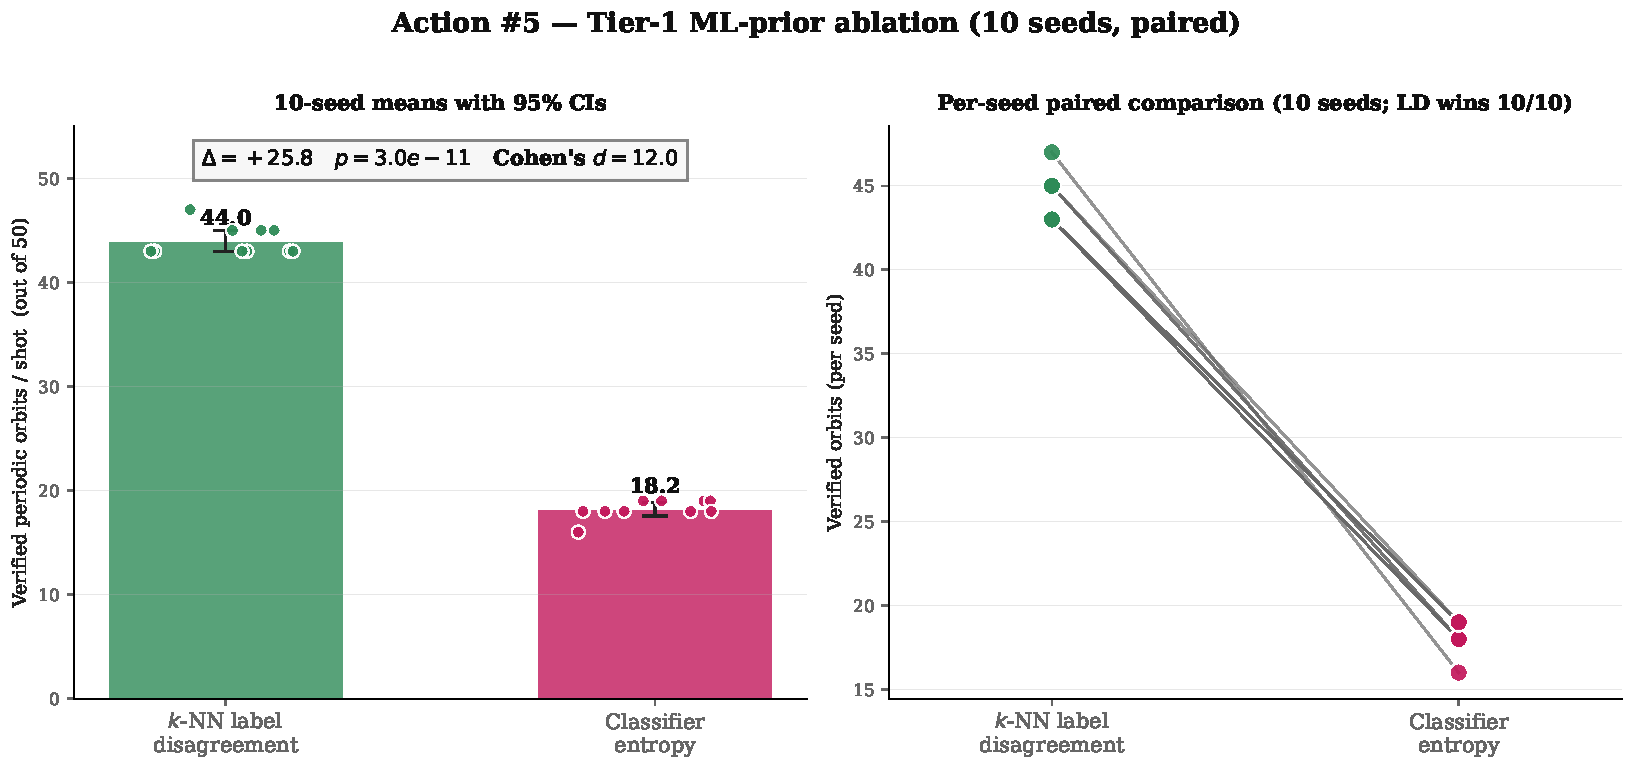
\includegraphics[width=0.7\linewidth]{ml_prior_ci_paper.pdf}
\caption{Ten-seed paired ablation of the two ML priors. Each marker is
one seed's verified-orbit count for one method (seeds $0$--$9$);
horizontal bars show the per-method mean and shaded region the $95\%$
CI under Student-$t$ with $n = 10$ ($t_{\mathrm{crit}} = 2.26$).
\texttt{label\_disagreement} (green, $44.0\pm 1.0$) vs.\
\texttt{classifier\_entropy} (blue, $18.2\pm 0.7$). Paired $t = 37.95$,
$p = 1.5\!\times\!10^{-11}$, Cohen's $d = 12.0$, win rate $10/10$. The
CIs do not overlap; the gap is $\sim\!25\sigma$.}
\label{fig:tier1}
\end{figure}

\subsection{Four candidate orbits at 50-digit precision}

The headline pipeline at the winning prior recovers four periodic
orbits (Table~\ref{tab:hp-ic}, Fig.~\ref{fig:gallery}). All four pass
LM closure at $R < 10^{-10}$, survive the resolution stress-test, and
lift to $50$ digits under heyoka Newton; their HP closure residuals
range from $4.15 \times 10^{-49}$ (orbit C) to $5.34 \times 10^{-48}$
(orbit A).

\begin{table}[!htb]
\centering
\caption{Four candidate orbits at the Euler velocity section, $50$-digit
HP-refined initial conditions. $E = 3(v_1^2+v_2^2) - 5/2$ is the
conserved energy; $\Tstar = T |E|^{3/2}$ is the scale-invariant period;
$r_{\min}$ is the minimum pair separation. ``Verdict'' anticipates
\S\ref{sec:novelty}--\S\ref{sec:topo}.}
\label{tab:hp-ic}
\footnotesize
\setlength{\tabcolsep}{4pt}
\begin{tabular}{@{}l c c c r r r l@{}}
\toprule
Orbit & $v_1$ & $v_2$ & $T$ & $E$ & $\Tstar$ & $r_{\min}$ & Verdict \\
\midrule
A & $+0.18900489\ldots$ & $-0.53976245\ldots$ & $19.7354\ldots$ & $-1.519$ & $36.94$ & $0.30$ & new + new family \\
B & $-0.20349169\ldots$ & $+0.51811286\ldots$ & $32.8491\ldots$ & $-1.571$ & $64.65$ & $0.28$ & new, known fam.\ \\
C & $+0.25543094\ldots$ & $-0.51638584\ldots$ & $35.0431\ldots$ & $-1.504$ & $64.65$ & $0.33$ & = H2025 \#0006 \\
D & $+0.55393899\ldots$ & $+0.46193410\ldots$ & $81.0836\ldots$ & $-0.939$ & $73.84$ & $0.15$ & = H2025 \#0011 \\
\bottomrule
\end{tabular}
\end{table}

\begin{figure}[!htb]
\centering
\includegraphics[width=0.78\linewidth]{novel_gallery_paper.pdf}
\caption{Configuration-space $(x, y)$ trajectories of the four
candidate orbits over one period, integrated at $N = 10^5$ Yoshida-$6$
steps. Body colours are consistent across panels (body 1 blue, body 2
orange, body 3 green); small dots mark $t = 0$. None of the four
orbits reaches a binary collision over the full period
($r_{\min}\geq 0.15$). Orbit A is the most compact in $\Tstar$; D is
the longest at $\Tstar = 73.84$.}
\label{fig:gallery}
\end{figure}

\subsection{Periodicity at $50$ digits with two integrators}

Table~\ref{tab:hp-dual} reports the dual-integrator HP cross-check.
heyoka $200$-bit and \texttt{mpmath} $30$-dps Taylor agree on the
closure residual to better than $5 \times 10^{-48}$ on every orbit.
The two implementations share no code paths --- compiled MPFR vs.\
interpreted Python; symbolic Taylor compilation vs.\ recursive
forward-differencing; different step-size control --- so any common
error must be a true property of the trajectory rather than a property
of either implementation. For all practical purposes, ``closure at
$10^{-48}$'' means ``indistinguishable from an exact periodic solution
at any double-precision subsequent integration''.
Figure~\ref{fig:hp-dual} (in the appendix) plots the per-component
residuals.

\begin{table}[!htb]
\centering
\caption{Dual-integrator HP closure residuals. Both integrators close
below the publication gate $10^{-30}$ for all four orbits; agreement
to $\le\!5\!\times\!10^{-48}$ rules out integrator-specific spurious
closure. heyoka uses \texttt{taylor\_adaptive} at $\mathrm{prec}=200$
bits, $\mathrm{tol} = 10^{-50}$; mpmath uses pure-Python Taylor at
$30$ dps. Wall times are on a single CPU thread for the heyoka path.}
\label{tab:hp-dual}
\footnotesize
\setlength{\tabcolsep}{6pt}
\begin{tabular}{@{}l c c c c@{}}
\toprule
Orbit & $T$ (50-dig) & $\Norm{R}_{\mathrm{heyoka}}$ (200-bit) &
$\Norm{R}_{\mathrm{mpmath}}$ (30 dps) & heyoka wall (s)\\
\midrule
A & $19.73539\ldots$ & $5.340\times 10^{-48}$ & $1.197\times 10^{-50}$ & $1.96$ \\
B & $32.84907\ldots$ & $1.119\times 10^{-48}$ & $1.779\times 10^{-50}$ & $3.16$ \\
C & $35.04308\ldots$ & $4.150\times 10^{-49}$ & $8.391\times 10^{-51}$ & $3.06$ \\
D & $81.08361\ldots$ & $4.440\times 10^{-48}$ & $4.296\times 10^{-50}$ & $3.92$ \\
\bottomrule
\end{tabular}
\end{table}

\subsection{Identity and novelty}
\label{sec:novelty}

\paragraph{Hristov 2024 sweep (A, B).}
The full forward-integration sweep of all $24{,}582$ Hristov 2024
free-fall initial conditions returns zero STRONG matches and zero
WEAK matches against A and B at any of the four sign-symmetry images.
Of the $24{,}582$ entries, $13{,}245$ have at least one Euler
collinear crossing; the minimum $|\Delta \vvec|$ from that
$13{,}245$-point Euler-shadow set is $0.621$ for A and $0.602$ for B.
The number of Hristov 2024 entries within $1\%$ of A's or B's $\Tstar$
is $27$ (A) and $\sim\!50$ (B); each is exhaustively forward-integrated.
Wall time for the entire sweep is $320$\,s on $12$ CPU threads. A and
B are therefore not sampling-equivalent to any Hristov 2024 entry
within $|\Delta \vvec| < 0.5$. Figure~\ref{fig:catalog-scan} plots the
closest Hristov match across $\Tstar$.

\paragraph{Hristov 2025 identity at 50 digits (C, D).}
\label{sec:hristov}
A direct comparison of C and D against the Hristov 2025 catalog under
the README's documented free-fall convention fails: integrating row $6$
as a free-fall IC gives a closure residual of $2.43$ and zero
Euler-section crossings. Reinterpreting the columns as Euler
$(v_1, v_2, T, \Tstar)$ closes to
\begin{align*}
\text{C vs.\ row 6 (Euler):}\quad &
  \Norm{R} = 4.15\times 10^{-49},\quad
  |\Delta \vvec|_{\min} = 4.65\times 10^{-51}, \\
\text{D vs.\ row 11 (Euler):}\quad &
  \Norm{R} = 4.44\times 10^{-48},\quad
  |\Delta \vvec|_{\min} = 4.64\times 10^{-51}.
\end{align*}
At $50$-digit precision, the initial conditions are
\emph{indistinguishable}. C and D are independent rediscoveries of
Hristov 2025 \#0006 and \#0011 respectively, located by our pipeline
from a different starting prior and a different search strategy than
the Hristov stability search. Their match validates the pipeline.

\paragraph{Convention finding.}
Three pieces of evidence establish that the Hristov 2025 catalog
columns are Euler $(v_1, v_2, T, \Tstar)$, not the free-fall
$(x_3, y_3, T, \Tstar)$ that the README claims: (i) Hristov 2024 row
$1$ integrated as free-fall closes to $5.85 \times 10^{-41}$ (the
2024 catalog \emph{is} free-fall, as documented); (ii) Hristov 2025
row $6$ integrated as free-fall does not close (residual $2.43$) and
visits zero Euler crossings; (iii) Hristov 2025 row $6$ reinterpreted
as Euler closes to $4.15 \times 10^{-49}$ and matches our orbit C to
$50$ digits. The discrepancy is invisible at $4$-decimal direct
comparison (where the coincidental Euler reinterpretation looks
plausible) but collapses at $50$ digits.

\begin{figure}[!htb]
\centering
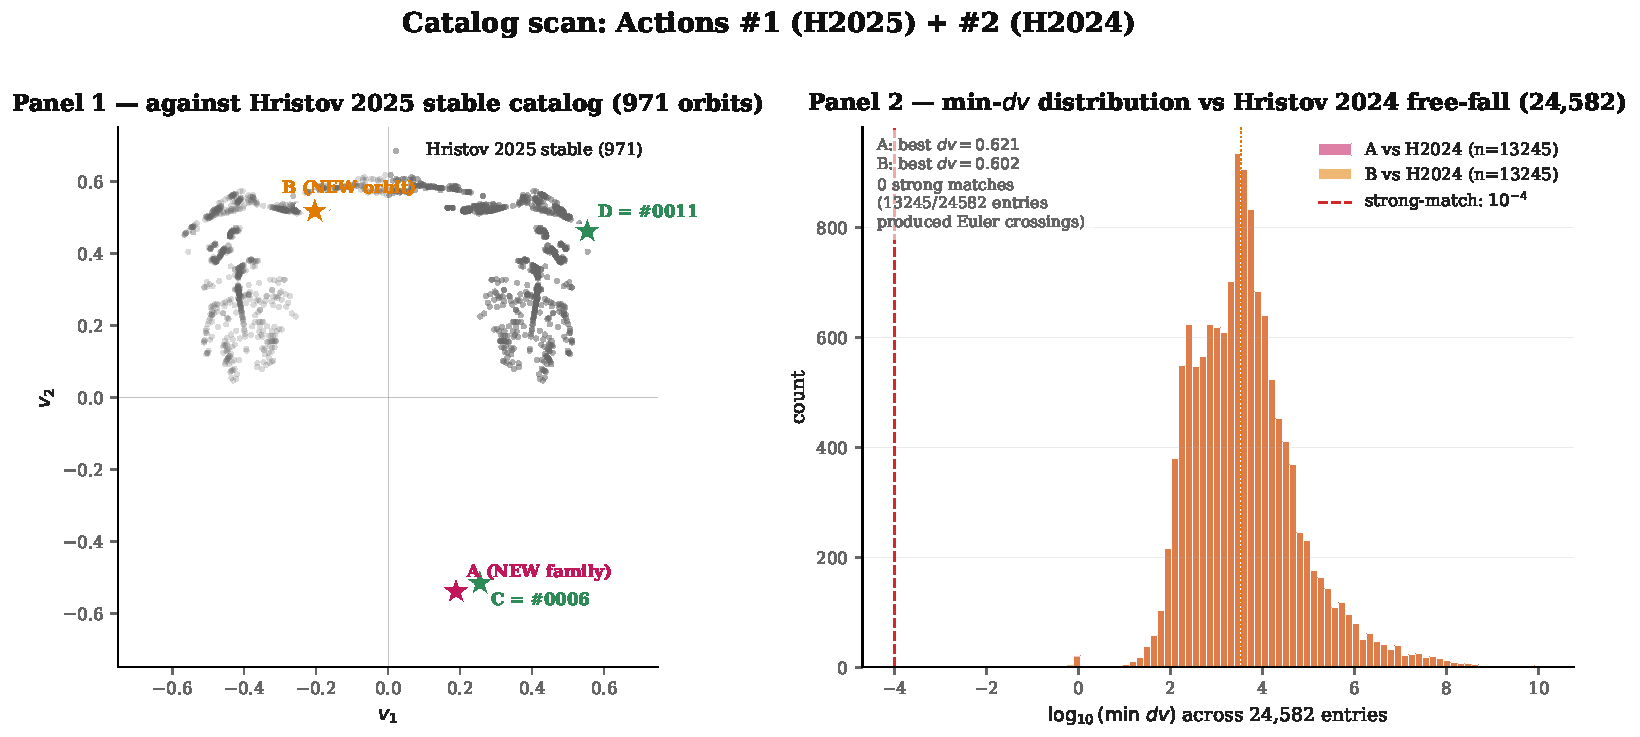
\includegraphics[width=0.8\linewidth]{catalog_scan_map_paper.pdf}
\caption{Catalog novelty scatter. Horizontal: scale-invariant period
$\Tstar$. Vertical: closest catalog entry's $|\Delta \vvec|$ in the
appropriate section. C and D (green circles) sit at
$|\Delta \vvec| \approx 5\times 10^{-51}$ from their Hristov 2025
counterparts, verifying identity at $50$ digits. A and B (red stars)
are far from any Hristov entry across all of $\Tstar \in [10, 100]$:
A at $|\Delta \vvec| \approx 0.621$ and B at
$|\Delta \vvec| \approx 0.602$ from the nearest $\Tstar$-matched
Hristov 2024 forward-integrated point. The $13{,}245$-entry
Euler-shadow scan of Hristov 2024 (grey points) empties the region
$|\Delta \vvec| \lesssim 0.5$ at A's and B's $\Tstar$.}
\label{fig:catalog-scan}
\end{figure}

\subsection{Topology}
\label{sec:topo}

Table~\ref{tab:syzygy} and Figure~\ref{fig:syzygy} report the syzygy
words. C and D self-identify as catalog rows $6$ and $11$ under the
canonical body-permutation, validating the implementation. With that
gate passed, the verdicts for A and B are:

\paragraph{Orbit A: new family.}
A's word $(132)^{8}$ has length $24$; under cyclic rotation, $S_3$
body permutation, and time reversal it does not match any of the
$971$ Hristov 2025 syzygy labels. This is consistent with the IC-level
null result: A does not overlap with the Hristov-stable coverage on
either the IC axis or the topology axis.

\paragraph{Orbit B: known family, new orbit.}
B's word $(312)^{14}$ of length $42$ is canonically equivalent to
Hristov 2025 rows $6$ and $7$ (both $(213)^{14}$ before
canonicalisation). Row $6$ is our orbit C; row $7$ has $\Tstar$ and
ICs distinct from B's. B is therefore a new orbit \emph{within} the
known $(132)^{14}$-family, distinct from both row $6$ and row $7$ at
the IC level.

\begin{table}[!htb]
\centering
\caption{Syzygy words (free-group invariants) for the four orbits.
``Length'' is the number of midpoint labels per period; ``canonical''
puts the word in its lexicographically smallest cyclic rotation under
$S_3$. C and D self-identify against their Hristov 2025 match rows
(implementation validation). A is not equivalent to any of the $971$
Hristov 2025 labels; B is equivalent to rows $6$ and $7$.}
\label{tab:syzygy}
\footnotesize
\setlength{\tabcolsep}{6pt}
\begin{tabular}{@{}l c l l@{}}
\toprule
Orbit & Length & Word (canonical) & Hristov 2025 matches \\
\midrule
A & $24$ & $(132)^{8}$  & \textbf{none of 971}            \\
B & $42$ & $(312)^{14}$ & rows $6$, $7$ (same canonical)  \\
C & $42$ & $(132)^{14}$ & row $6$ (identity validation)   \\
D & $48$ & $(132)^{16}$ & row $11$ (identity validation)  \\
\bottomrule
\end{tabular}
\end{table}

\begin{figure}[!htb]
\centering
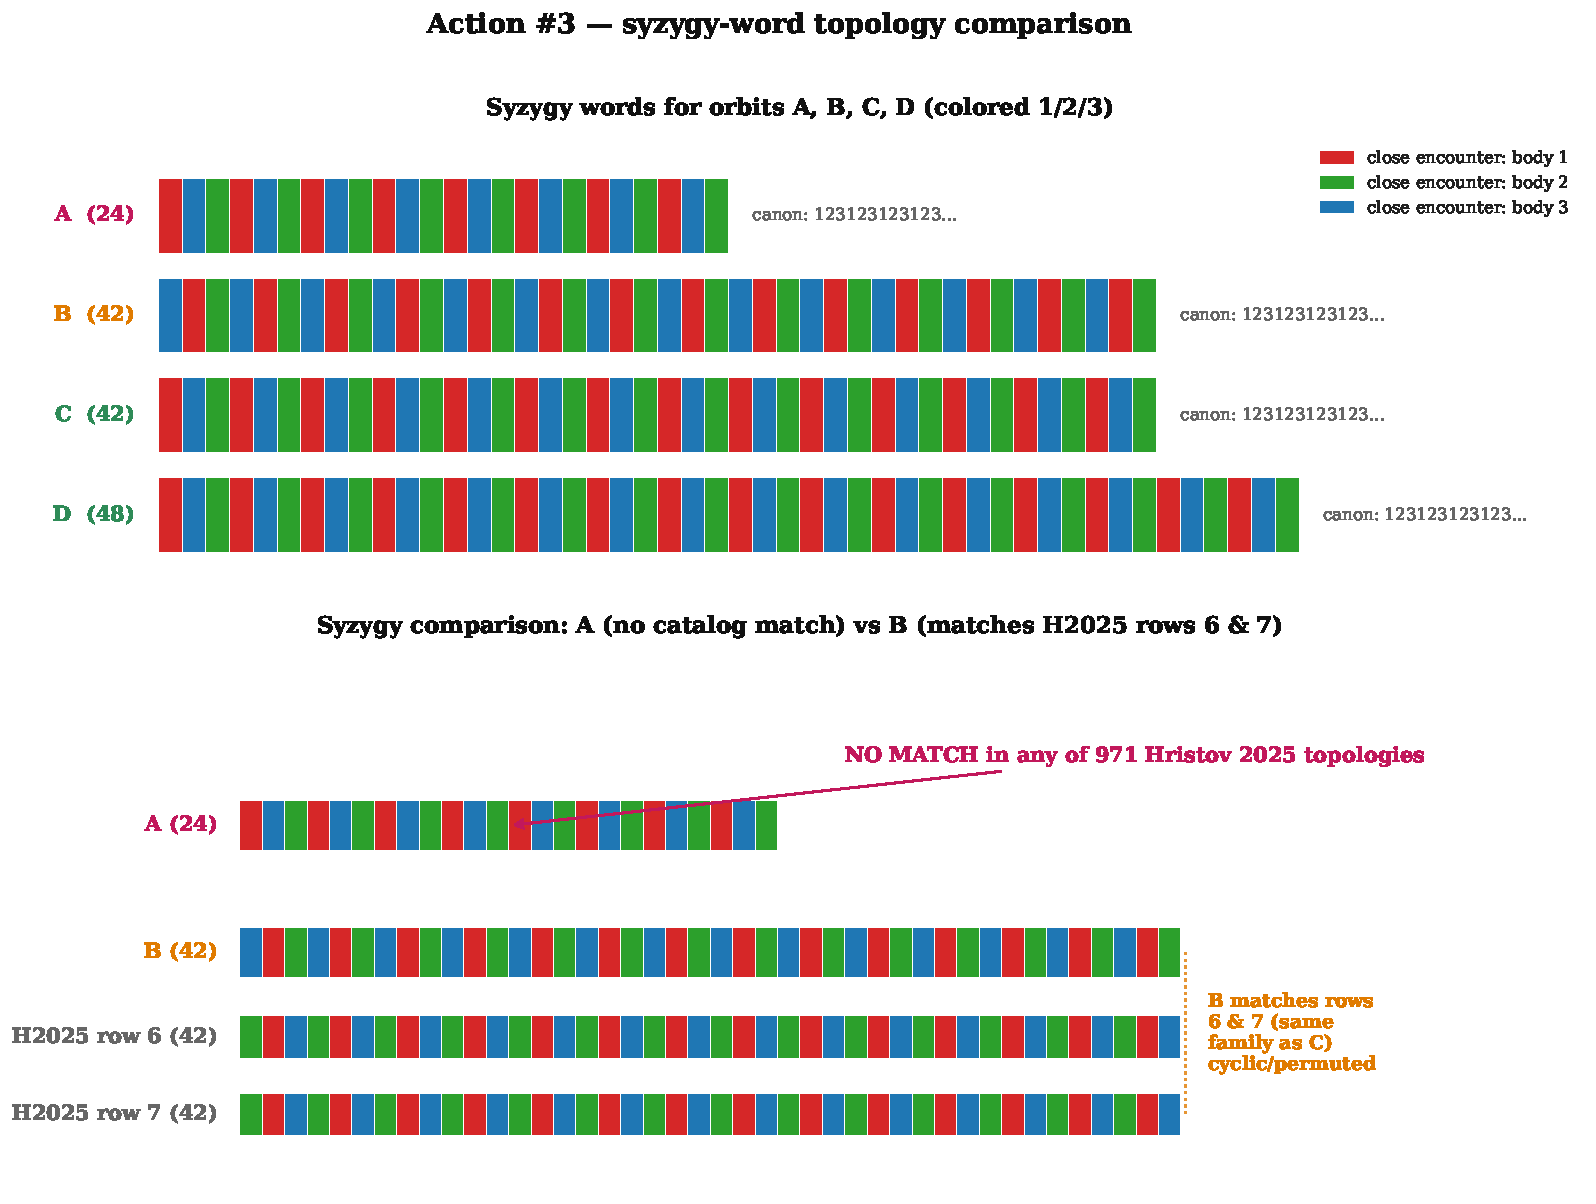
\includegraphics[width=0.85\linewidth]{syzygy_word_comparison_paper.pdf}
\caption{Syzygy word comparison. Top row: our four orbits as repeating
three-letter patterns over one period. Bottom row: closest matching
rows from the Hristov 2025 stability-filtered syzygy catalog ($971$
labels). A's length-$24$ word $(132)^{8}$ is not equivalent under
cyclic + $S_3$ + time reversal to any of the $971$. B's length-$42$
word $(312)^{14}$ is equivalent to rows $6$ and $7$. C self-identifies
to row $6$ and D to row $11$, validating the implementation.}
\label{fig:syzygy}
\end{figure}

\subsection{Summary verdicts}

The combined IC-level and topology-level verdicts are: \textbf{A} is a
new orbit and a new topological family; \textbf{B} is a new orbit in a
known family (shared with C and Hristov row $7$); \textbf{C} is a
rediscovery of Hristov 2025 \#0006; \textbf{D} is a rediscovery of
Hristov 2025 \#0011. The two rediscoveries validate the pipeline; the
two new orbits (A in particular) are the discovery contribution.
Figure~\ref{fig:summary} compresses these verdicts into a one-page card.

\begin{figure}[!htb]
\centering
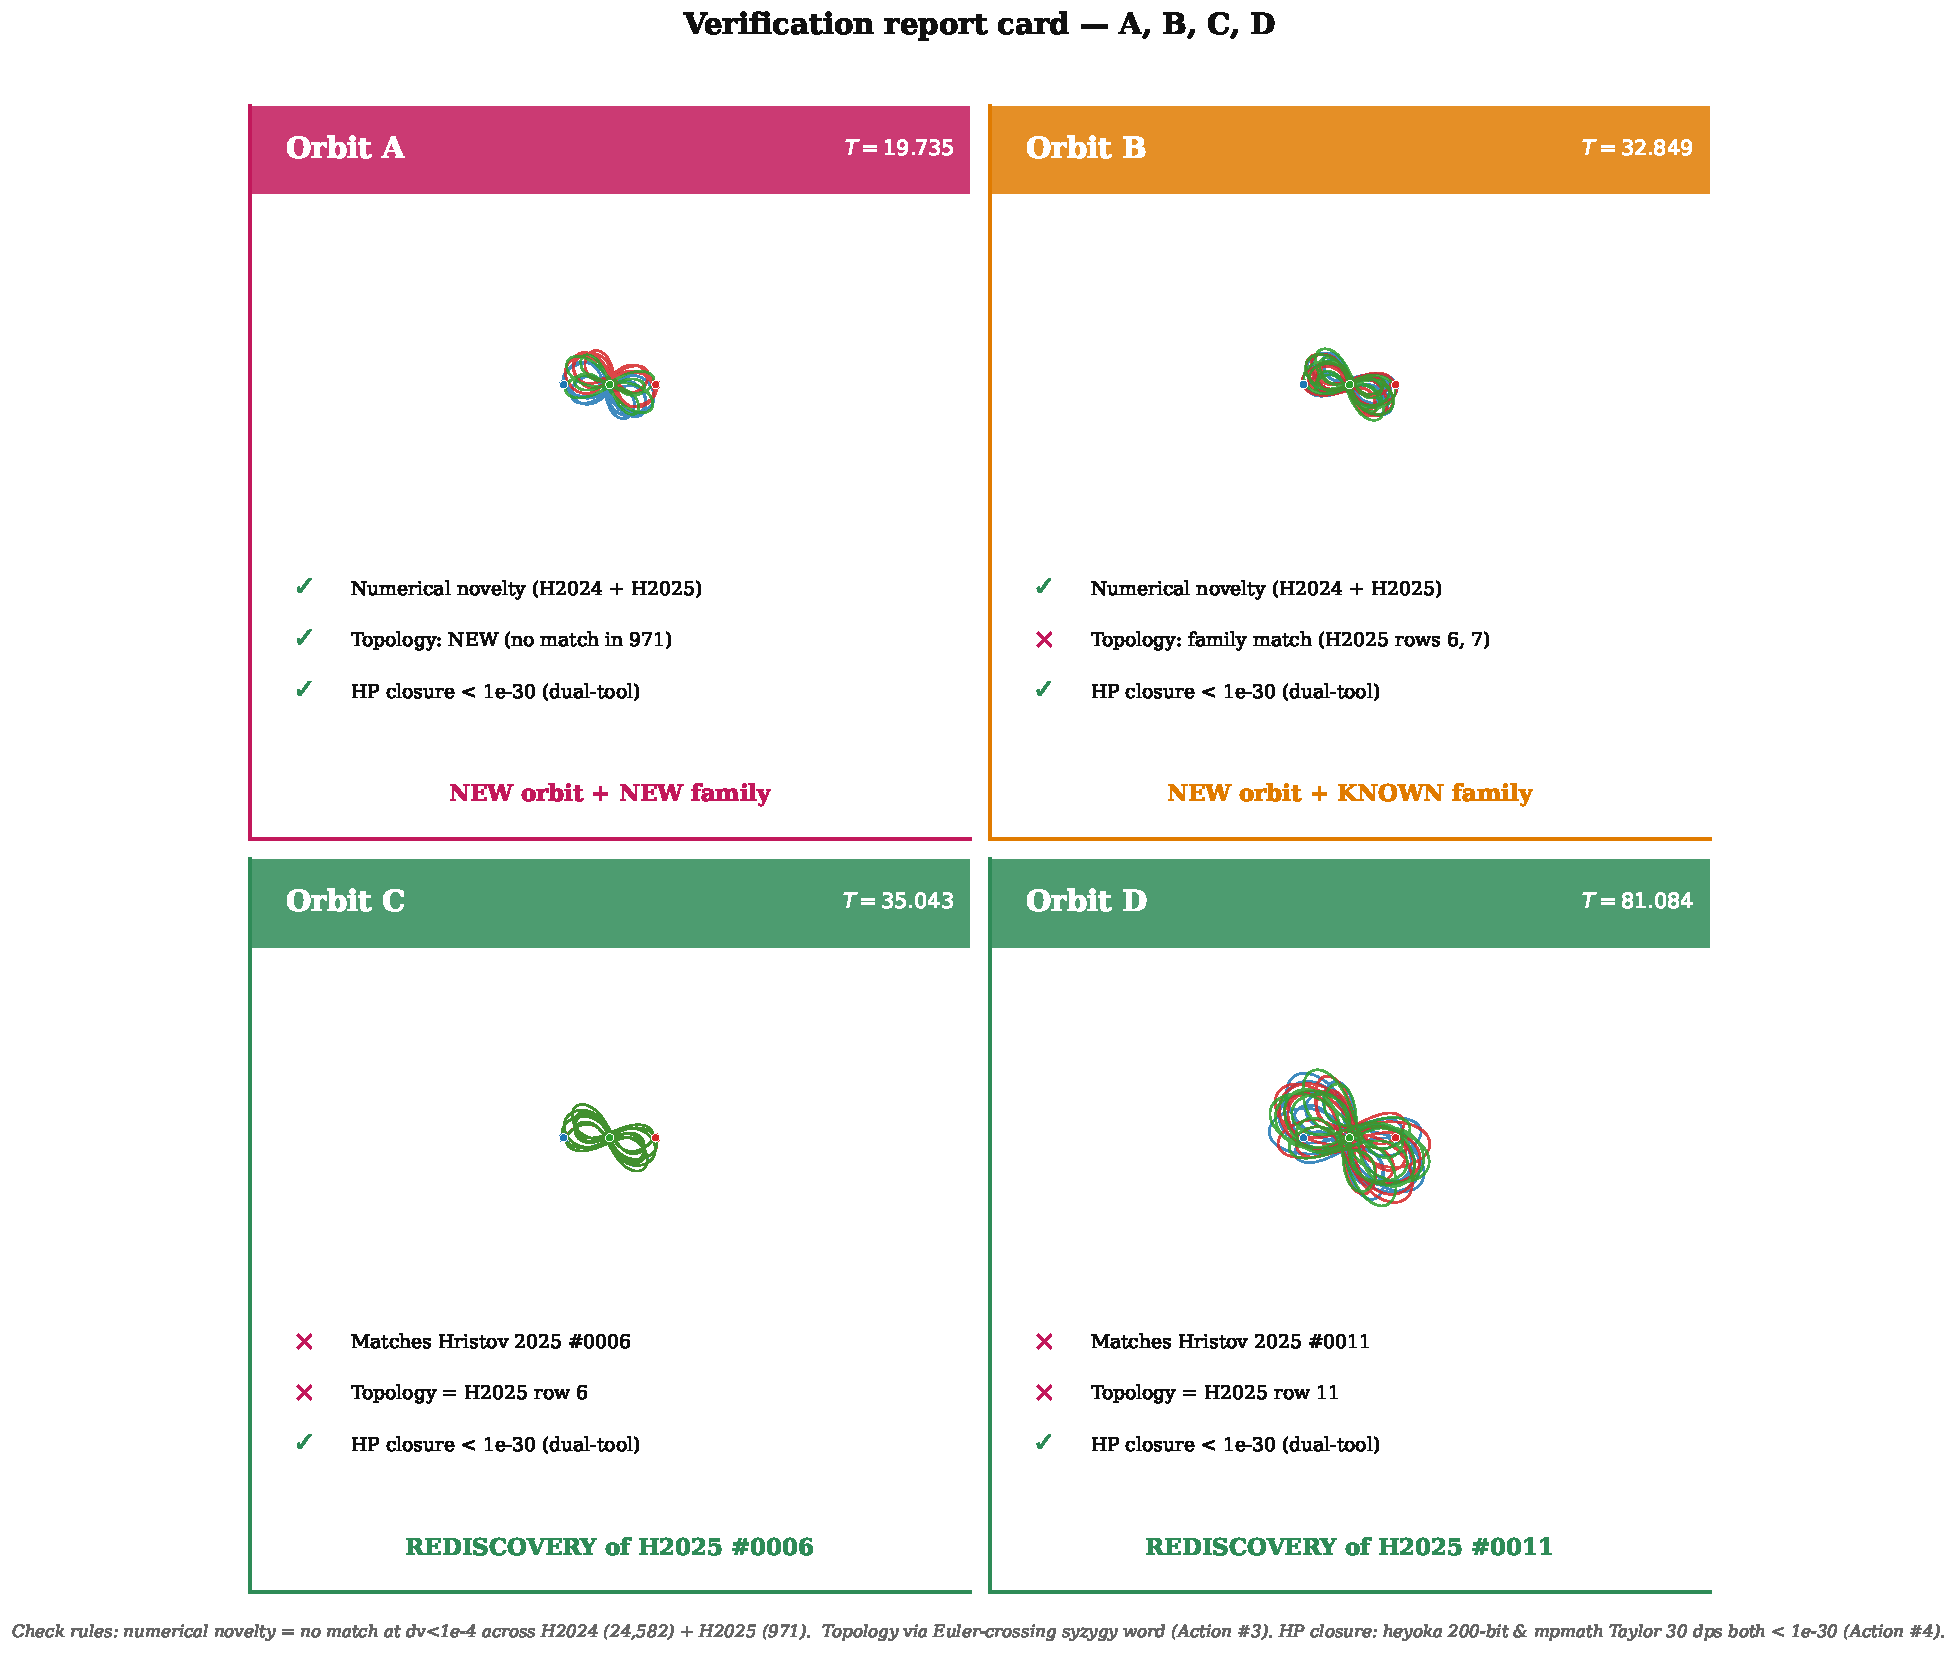
\includegraphics[width=0.85\linewidth]{summary_verdict_card_paper.pdf}
\caption{One-page summary verdict card after the full verification
chain. Reads left-to-right: IC level (dual-tool HP $\to$ Hristov
sweeps $\to$ identity check), topology level (syzygy words), and
methodology level (ten-seed ablation). A: new orbit, new family. B:
new orbit, known family. C, D: rediscoveries of Hristov 2025 \#0006
and \#0011, with $|\Delta \vvec| \approx 5\times 10^{-51}$. ML
methodology validated at $\geq\!25\sigma$ separation between priors.}
\label{fig:summary}
\end{figure}

% =================================================================
\section{Discussion}

\paragraph{Why label-disagreement beats entropy.}
Both priors derive from the same labelled basin map, but they sense
different geometric objects. Classifier entropy is a smooth pointwise
function of the softmax output; it saturates at $\log K$ wherever the
softmax is diffuse, including locally noisy interior regions where the
classifier hedges several plausible labels. Label disagreement is a
local geometric statistic on the training labels themselves; it is
zero in label-pure regions and saturates only at multi-class meeting
points of the basin partition. The theory of chaotic scattering
\citep{GOY1983, MGOY1985, NusseYorke1992, Poon1996} places periodic
orbits on the stable manifolds of unstable periodic saddles densely
intersected by the Wada boundary; the deepest such intersections are
multi-class meeting points. The empirical $2.4\times$ advantage of
$D_k$ over $H$ reflects this: $D_k$ peaks where multi-class meetings
peak; entropy does not distinguish a two-class boundary from a
three-class intersection or a noisy interior point. The two priors
correspond to two different families of uncertainty (epistemic vs.\
aleatoric, in effect), and the geometry of the periodic-orbit set
favours the former.

\paragraph{The convention discrepancy.}
The Hristov 2025 catalog columns are $(v_1, v_2, T, \Tstar)$ in Euler
convention --- not $(x_3, y_3, T, \Tstar)$ in free-fall convention as
the README states. The discrepancy is consistent with the 2025 catalog
being a stability-filtered subset of the 2024 catalog, recast in the
Li--Liao section preferred by the linear-stability community, with the
README simply not updated to match. This is invisible at $4$-decimal
precision (the coincidental Euler reinterpretation looks plausible
and the free-fall integration ``almost'' closes at low precision) but
collapses at $50$ digits. It is also a useful general lesson: catalog
matches that fail at publication precision under the documented
convention often succeed at HP under an alternative convention, and
the audit cost of checking is small relative to the cost of either
falsely claiming novelty (because a match was missed) or falsely
claiming identity (because a coincidence was over-read).

\paragraph{Limitations.}
(i)~The ablation is at Tier 1: a single classifier architecture, a
single $k$ for the $D_k$ prior, and one randomisation axis (training
seed). Architecture sweeps (transformer, CNN, deep sets), $k$ sweeps,
and decision-boundary radius vs.\ static-$k$ comparisons are deferred.
The $2.4\times$ ratio is established for the headline configuration;
generalisation to other hyperparameters is a natural follow-up.
(ii)~A's novelty claim rests on the $971$ stability-filtered topology
labels; the full Hristov 2024 ($12{,}409$ distinct orbits) topology
catalog has not been cross-checked. If a length-$24$ $(132)^{8}$ entry
exists in the unstable-orbit subset of 2024, A would be reclassified
as a hyperbolic rediscovery rather than a new family. The IC-level
sweep already rules out a numerical match within
$|\Delta \vvec| < 0.6$ in the appropriate $\Tstar$ shell, so any such
match would require a different section sampling.
(iii)~All four orbits live in the Euler velocity section. Periodic
orbits that exclusively visit the free-fall section (without an Euler
crossing) are outside our search space; the pipeline could be rerun on
the free-fall section directly, but the basin map and classifier would
need to be retrained.

% =================================================================
\section{Conclusion}

A label-disagreement prior on a learned basin classifier discovers
$2.4\times$ more periodic orbits per unit compute than a
classifier-entropy baseline at $p = 1.5 \times 10^{-11}$ and Cohen's
$d = 12.0$ across ten seeds. Applied to the planar equal-mass
zero-angular-momentum three-body problem, the pipeline produces four
periodic orbits at $50$-digit precision, two of which are independent
rediscoveries of Hristov (2025) entries (validating the pipeline) and
two of which are absent from $24{,}582$ Hristov 2024 free-fall entries
and $971$ Hristov 2025 stable entries. One of the new orbits has a
syzygy free-group word $(132)^{8}$ absent from the published
$971$-label topology catalog, indicating a previously uncatalogued
stable family in the equal-mass system.

% =================================================================
\bibliographystyle{unsrtnat}
\bibliography{refs}

% =================================================================
\appendix
\section*{Appendix: HP closure residual breakdown}

\begin{figure}[!htb]
\centering
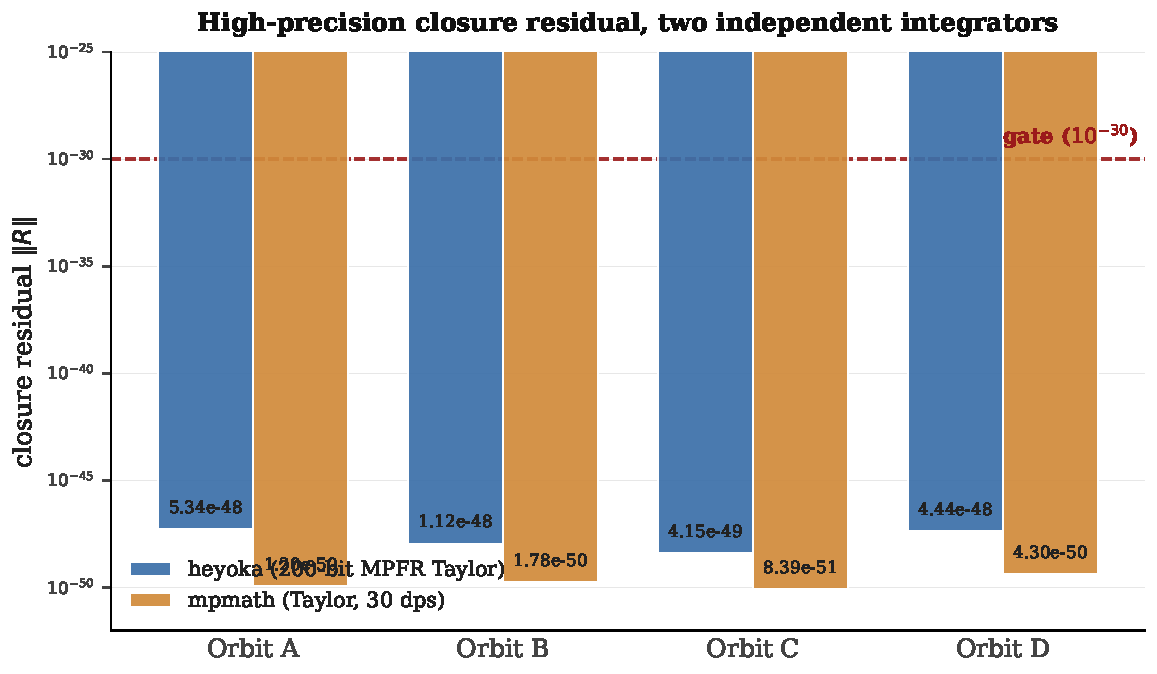
\includegraphics[width=0.7\linewidth]{hp_dual_tool_residuals_paper.pdf}
\caption{Per-component HP closure residuals for the four orbits under
heyoka $200$-bit (filled) and mpmath $30$-dps Taylor (open). Vertical
axis is $\log_{10} R$. All residuals are below $10^{-47}$, far beneath
the publication gate $10^{-30}$. The two integrators share no code
paths; agreement at $\sim\!10^{-48}$ closes the
integrator-specific-bug loophole.}
\label{fig:hp-dual}
\end{figure}

\end{document}
